% Verifier-Anchored Reinforcement Learning over a Frozen LLM
% 10-minute talk. Build: latexmk -pdf 2026-06-23-verifier-anchored-rl-talk.tex
% Theme: metropolis (TeX Live package beamertheme-metropolis). Compiles with
% pdflatex; xelatex/lualatex give the Fira font if installed.
% Speaker notes are attached per frame via \note{}; to present them, uncomment
% the show-notes option below.
\documentclass[aspectratio=169]{beamer}

\usetheme{metropolis}
\metroset{block=fill}

\usepackage{amsmath,amssymb}
\usepackage{booktabs}
\usepackage{tikz}
\usetikzlibrary{arrows.meta,positioning,calc}

% Presenter build: define \shownotes to put speaker notes on a second screen
% (each page becomes slide + notes side-by-side, which pdfpc/pympress split
% across the presenter and audience displays). Default build = clean audience
% deck. Build both with the Makefile (make audience ; make presenter), or:
%   latexmk -pdf -usepretex='\def\shownotes{}' -jobname=<name>-presenter <file>.tex
\ifdefined\shownotes
  \setbeameroption{show notes on second screen=right}
\fi

% Shorthand for the learned/target quantities (keeps slides terse and consistent).
\newcommand{\pitheta}{\pi_\theta}
\newcommand{\Qpsi}{Q_\psi}
\newcommand{\piMCTS}{\pi_{\mathrm{MCTS}}}
\newcommand{\QMCTS}{Q_{\mathrm{MCTS}}}
\newcommand{\verbword}[1]{\texttt{#1}}

\title{Teaching a Small Model to Deliberate}
\subtitle{Verifier-Anchored Reinforcement Learning over a Frozen LLM}
\date{2026}
\author{}

\begin{document}

\maketitle
\note{This is a reinforcement-learning talk. The central object is an agent with
a small action-value function over a structured state, trained against rewards a
deterministic verifier supplies. Keep that frame: everything else, MCTS included,
is machinery in service of learning a small, fast policy.}

% ---------------------------------------------------------------------------
\section{Motivation}

\begin{frame}{The pain: cheap models, expensive reasoning}
  \begin{itemize}
    \item Small 1--7B models are fast and deployable, but lag on GSM8K and MATH
    \item The gap is widest exactly where answers are checkable by a non-LLM verifier
    \item Test-time search (best-of-$N$, self-consistency, MCTS) helps, but is
          \alert{amnesiac}: every query pays full cost again, nothing is distilled back
    \item The question: can we close the gap \emph{without growing the model}?
  \end{itemize}
  \note{Small models are what we want to deploy, but they reason poorly across
  steps. Inference-time search patches the symptom and never learns from it. We
  want to turn that search into a teacher and learn a small policy, paying the
  search cost once during training rather than forever at inference.}
\end{frame}

\begin{frame}{And learned rewards get gamed}
  \begin{itemize}
    \item Dense \emph{learned} reward models are seductive but open a Goodhart attack surface
    \item Under enough optimization pressure, the policy converges on the proxy's defects
    \item Our anchor: a deterministic \alert{non-LLM verifier} (SymPy equality, unit tests, Lean type-check)
    \item A signal enters the reward channel only if it is an objective proposition a program can check
  \end{itemize}
  \note{The core reward-design commitment is an asymmetry: only verifier-checkable
  propositions may form rewards and Bellman backups; learned-aesthetic classifiers
  may enter only as search priors, never as reward. Keeping reward verifier-anchored
  rather than learned reduces the Goodhart attack surface by construction.}
\end{frame}

\begin{frame}{Thesis}
  \begin{enumerate}
    \item Freeze the base LLM; learn small heads $\pitheta,\ \Qpsi$ over a structured state
    \item Cast LLM deliberation on verifiable tasks as \alert{approximate $Q$-learning over an induced context MDP}
    \item Reward is verifier-anchored, not a learned critic
    \item MCTS is a sample-efficient \emph{policy-improvement operator} that supplies
          stronger training targets, \alert{not} the central algorithm
  \end{enumerate}
  \note{The whole talk in one slide. The learnable object is the agent and its
  action-value function, trained by approximate Q-learning of the DQN lineage.
  Tree search is one mechanism for producing better samples and stronger targets;
  it is subordinate to the learning. Because the LLM is frozen, any measured
  improvement is attributable to the heads and the search procedure.}
\end{frame}

% ---------------------------------------------------------------------------
\section{The setup: an induced context MDP}

\begin{frame}{The induced context MDP}
  \begin{itemize}
    \item State $s$: a structured reasoning context (not raw token soup)
    \item Actions $A$: seven coarse cognitive verbs, $|A| = 7$
    \item Transition $P$: frozen LLM $+$ prompt template samples the next state; non-enumerable
    \item Reward $R$: ground-truth terminal $+1/-1$ from the verifier; small capped intermediate shaping
    \item Controller observes only \emph{sampled} transitions: model-free RL with the LLM as the environment
  \end{itemize}
  \note{The next state is whatever the LLM continuation plus a lossy parser
  produce, so the transition kernel is neither enumerable nor closed-form. The
  controller never sums over next states; it only observes samples. That single
  fact later forces sampled chance nodes as the only honest estimator of the
  Bellman inner expectation.}
\end{frame}

\begin{frame}{Structured state: a shell the LLM fills}
  \begin{itemize}
    \item Slots: problem $P$, Facts, open/closed Subgoals, Hypotheses, verifier log, committed answer, depth
    \item Load-bearing split: \textbf{Fact} (``I have proven this'') vs \textbf{Hypothesis} (``I think this is true'')
    \item Avoids two failure modes: raw tokens (no inductive bias) and one opaque embedding (no action masking)
    \item Serialized with structural markers: \verbword{[FACT]}, \verbword{[HYPOTHESIS]}, \verbword{[VERIFIER\_CALL]}, \verbword{[STATE\_END]}
  \end{itemize}
  \note{The schema makes the Markov bet explicit. Fact-versus-Hypothesis is the
  most important design choice: tentative claims kept separate from verified ones,
  which is what deliberation needs. The state is embedded as the frozen LLM's
  hidden state at the [STATE\_END] sentinel.}
\end{frame}

\begin{frame}{Actions: seven cognitive verbs}
  \begin{block}{$A = \{$ \verbword{DECOMPOSE}, \verbword{COMPUTE\_SUBEXPR}, \verbword{FORM\_HYPOTHESIS}, \verbword{CHECK\_CASE}, \verbword{INVOKE\_VERIFIER}, \verbword{BACKTRACK}, \verbword{COMMIT\_ANSWER} $\}$}
  \end{block}
  \begin{itemize}
    \item Only the \emph{verb} is categorical; the LLM verb-instantiator generates the target id and content
    \item Action space stays cardinality-7 regardless of tree depth; a state-conditioned mask gates illegal verbs
    \item \verbword{INVOKE\_VERIFIER} is a first-class budgeted move, not a post-hoc parser pass
  \end{itemize}
  \note{Verbs are mostly realized as prompting templates the frozen base model
  instantiates, but not necessarily only prompts. Keeping the verb categorical
  gives the Q-head a fixed output and search a stable branching factor. Making
  InvokeVerifier a callable verb makes the verifier first-class deliberation the
  agent learns to budget.}
\end{frame}

\begin{frame}{A concrete trace (GSM8K)}
  \small
  \textit{P: ``A store sold 7 boxes with 6 pencils each. How many pencils?''}
  \begin{enumerate}
    \item \verbword{DECOMPOSE} \texttt{sg\_root}, then \verbword{FORM\_HYPOTHESIS}: \texttt{hyp\_1} $=$ ``the total is 42'' (tentative)
    \item \verbword{COMPUTE\_SUBEXPR} ``$7\times 6$'' $\to 42$, added as a derived Fact
    \item \verbword{INVOKE\_VERIFIER} on \texttt{hyp\_1} (SymPy) $\to$ confirmed; \texttt{hyp\_1} promoted to Fact ($+0.05$, capped)
    \item \verbword{COMMIT\_ANSWER} ``42'' $\to$ terminal verifier check $\to$ reward $+1$
  \end{enumerate}
  \note{This single trace is the entire RL story made concrete: state, verb-actions,
  sampled transitions, verifier reward. The small intermediate reward for a
  first-time successful verifier promotion is hard-capped so it cannot be farmed
  above the terminal magnitude. At inference $B{=}0$ walks this greedily; $B{>}0$
  runs MCTS to refine the verb choices.}
\end{frame}

% ---------------------------------------------------------------------------
\section{The learner}

\begin{frame}{Architecture: frozen LLM, tiny trainable heads}
  \begin{itemize}
    \item One frozen base LLM is \emph{both} encoder and stochastic transition/generator (one forward, not two)
    \item State embedding $=$ hidden state at \verbword{[STATE\_END]}; a small adapter MLP
    \item Multi-head $\Qpsi(s,a)$ over the 7 verbs, plus a policy-prior head $\pitheta$ sharing the adapter
    \item Total trainable params \alert{under 5M}: 2--3 orders of magnitude smaller than the frozen LLM
    \item Approximate $Q$-learning: replay buffer, target net synced every $N_{\mathrm{sync}}$, prioritized by TD error
  \end{itemize}
  \note{A single LLM forward yields both the state embedding and the
  verb-instantiator's continuation, which makes the shared-encoder design cheap.
  We train only the adapter and heads. Because the base never moves,
  representation drift is bounded and any gain is attributable to heads and search,
  not to fine-tuning the LLM.}
\end{frame}

\begin{frame}{Offline by design: learn from any trajectory}
  \begin{itemize}
    \item $Q$-learning is \alert{off-policy}: the $\max$ bootstrap refers to the greedy continuation, not the behavior policy
    \item So the learner can train from \emph{any} trajectories covering the state-action space
    \item Sources: its own runs, other models' runs, logged production data, human demonstrations
    \item Decouples data collection from learning: a genuine strength, not a limitation
    \item $\QMCTS$ targets are stored \emph{with} each replay sample, so stale entries do not break correctness
  \end{itemize}
  \note{Off-policy learning is what makes MCTS-guided collection, or any other
  collection, compatible with the learning rule. The quiet superpower: data source
  and learner are decoupled. It also sets up online continual learning, since
  deployment traffic is just one more source of off-policy experience.}
\end{frame}

\begin{frame}{MCTS as a policy-improvement operator (not the star)}
  \begin{itemize}
    \item The heads encode \emph{average} behavior; MCTS spends compute \emph{locally} on this state
    \item PUCT, with the learned policy as prior and $\Qpsi$ as leaf value:
  \end{itemize}
  \[
    a^\star = \arg\max_a\ \widehat{Q}(s,a) \;+\; c_{\mathrm{puct}}\, \pitheta(a\mid s)\,
      \frac{\sqrt{N(s)}}{1 + N(s,a)}
  \]
  \begin{itemize}
    \item Decision/chance-node (afterstate) split; the chance-node mean is an honest estimator of the Bellman inner expectation:
  \end{itemize}
  \[
    \frac{W(s,a)}{N(s,a)} \;\approx\; \sum_{s'} P(s'\mid s,a)\,\bigl[R(s,a,s') + \gamma V(s')\bigr]
  \]
  \centering Output: stronger targets \;$\piMCTS$\; (visit counts) and \;$\QMCTS$\; (chance-node $Q$).
  \note{MCTS enters as a policy-improvement operator: given current estimates it
  produces locally improved ones at a query state, replacing the intractable
  Bellman sum with sampled rollouts. The sampled chance node is the only available
  estimator of the inner expectation. The afterstate bifurcation is borrowed
  (Stochastic MuZero), not claimed as novel.}
\end{frame}

\begin{frame}{The self-reinforcing expert-iteration loop}
  \begin{columns}[T]
    \begin{column}{0.54\textwidth}
      \begin{itemize}
        \item Distill $\piMCTS$ into the policy head ($\mathcal{L}_\pi$, cross-entropy)
        \item Regress $\Qpsi$ onto $\QMCTS$, used \emph{in place of} single-sample Bellman targets
        \item $\mathcal{L}_{\mathrm{total}} = \underbrace{(\Qpsi - \QMCTS)^2}_{\mathcal{L}_Q} + \lambda\,\mathcal{L}_\pi$
        \item Fast vs slow: the heads are System 1, MCTS is System 2; training shifts competence into System 1
      \end{itemize}
    \end{column}
    \begin{column}{0.46\textwidth}
      \centering
      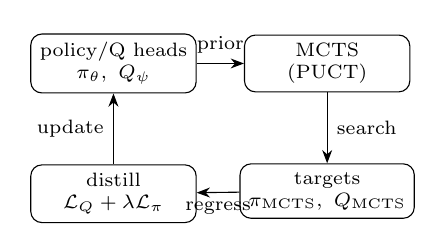
\begin{tikzpicture}[
          node distance=9mm and 6mm, >=Stealth, font=\scriptsize,
          box/.style={draw, rounded corners, align=center, inner sep=3pt, minimum width=21mm}]
        \node[box] (pol) {policy/Q heads\\$\pitheta,\ \Qpsi$};
        \node[box, right=of pol] (search) {MCTS\\(PUCT)};
        \node[box, below=of search] (tgt) {targets\\$\piMCTS,\ \QMCTS$};
        \node[box, below=of pol] (dist) {distill\\$\mathcal{L}_Q + \lambda\mathcal{L}_\pi$};
        \draw[->] (pol) -- node[above]{prior} (search);
        \draw[->] (search) -- node[right]{search} (tgt);
        \draw[->] (tgt) -- node[below]{regress} (dist);
        \draw[->] (dist) -- node[left]{update} (pol);
      \end{tikzpicture}
    \end{column}
  \end{columns}
  \note{The same approximate Q-learning update runs; only the targets get better,
  because they average over search-guided trajectories instead of single samples.
  This is AlphaZero's expert-iteration structure, inverted: the agent and its Q are
  the center, search is subordinate machinery for sample efficiency.}
\end{frame}

\begin{frame}{Reward hacking: a verifier is necessary, not sufficient}
  \begin{itemize}
    \item Goodhart is the classic RL failure: optimize a mis-specified reward, get gamed behavior that scores well and reasons badly
    \item A non-LLM verifier removes the \emph{learned}-reward attack surface, but a poorly specified verifier reward is still gameable
    \item We red-teamed our own intermediate shaping reward and found a farm: verify content-free tautologies or self-authored claims for free reward
  \end{itemize}
  \begin{alertblock}{Fix by construction, not by patch}
    Tie the rewarded check to the target claim; reward only the \emph{first} success per target;
    hard-cap cumulative intermediate reward at $\tfrac{1}{5}$ of the terminal magnitude $\Rightarrow$
    the ground-truth terminal verifier always dominates, so farming is \emph{bounded}, not merely discouraged.
  \end{alertblock}
  \note{The honest slide. A verifiable reward is necessary but not sufficient: a
  badly specified shaping term is still hackable. We caught exactly this via
  adversarial review, the agent earning the small reward by verifying trivially
  true but irrelevant self-authored claims. The fix is structural: tie to target,
  reward each target once, cap the cumulative shaping well below the terminal so no
  farm can rival actually solving. Red-teaming the reward is part of the method.}
\end{frame}

% ---------------------------------------------------------------------------
\section{Inference and deployment}

\begin{frame}{The compute knob $B$: fast by default, think harder on demand}
  \begin{columns}[T]
    \begin{column}{0.5\textwidth}
      \begin{block}{$B = 0$ (fast)}
        masked $\arg\max$ over $\Qpsi$; one LLM forward per decision; constant latency
      \end{block}
    \end{column}
    \begin{column}{0.5\textwidth}
      \begin{block}{$B > 0$ (search)}
        run PUCT MCTS for $B$ simulations; sample the visit-count policy
      \end{block}
    \end{column}
  \end{columns}
  \vspace{0.5em}
  \begin{itemize}
    \item Same trained $\Qpsi$ and $\pitheta$ in both modes; one dial traces a compute-vs-accuracy frontier, no retraining
    \item Fast mode is competitive precisely because the heads were distilled from MCTS targets
  \end{itemize}
  \note{Two modes, not two algorithms: the same learned actor with different
  amounts of search on top. The search budget becomes a continuous dial the user
  controls at inference. Because $\Qpsi \approx \QMCTS$ and $\pitheta \approx
  \piMCTS$ at the training budget, $B{=}0$ already carries much of the benefit.}
\end{frame}

\begin{frame}{Online continuous learning in deployment}
  \begin{itemize}
    \item Because it is off-policy and feedback-anchored, learning need not stop at deploy
    \item Any verifier-style signal keeps it improving, including user thumbs up/down
    \item The signal must stay a \emph{structural check}, never a learned classifier in the Bellman target
    \item Adapter-tier separation: per-user adapters absorb idiosyncratic feedback; the global adapter accepts only changes that survive aggregation
  \end{itemize}
  \centering\emph{A model that gets better the longer it is used.}
  \note{The small adapter MLP is the plug-in point for deployment learning. The
  tiering keeps any one user's signals from dominating global updates. The verifier
  stays the trusted anchor throughout, which bounds Goodhart drift even as feedback
  arrives from the wild.}
\end{frame}

% ---------------------------------------------------------------------------
\section{Positioning and evaluation}

\begin{frame}{Positioning and defensible novelty}
  \begin{itemize}
    \item \textbf{Search-and-learning in games} (AlphaZero, expert iteration): we \alert{invert} it, agent and $\Qpsi$ central, search optional
    \item \textbf{Verifier-anchored reasoning} (PRMs, AlphaCode, AlphaProof, DeepSeek-R1): the verifier-vs-aesthetic asymmetry is load-bearing; \verbword{INVOKE\_VERIFIER} is a callable verb
    \item \textbf{VerifierQ}: verifier-as-\emph{action} not verifier-as-$Q$; online distilled targets not fixed-dataset fitting; categorical multi-head $Q$
    \item \textbf{rStar-Math}: same family, but ours is a structured-state seven-verb MDP
    \item \textbf{vs STaR / ReST-EM / Math-Shepherd}: we distill per-step $\QMCTS$ as a genuine Bellman target, not trajectory-level or a process-reward model
  \end{itemize}
  \note{We inherit AlphaZero's joint search-and-learning structure but invert its
  center, making non-search baselines first-class. Against the closest Q-learning
  core, VerifierQ, we differ on three concrete axes. We do not claim the afterstate
  bifurcation as novel; novelty is its application to the non-enumerable
  LLM-induced transition.}
\end{frame}

\begin{frame}{How we will evaluate (the plan, not results)}
  \begin{itemize}
    \item Benchmarks GSM8K and MATH; a baseline grid fixed in advance: base-greedy, best-of-$N$, self-consistency, STaR/ReST-EM, AlphaZero-for-reasoning, PRM-guided
    \item \alert{Pre-registered} falsifiable hypotheses and the headline frontier figure committed \emph{before} any training
    \item $\geq 3$ training seeds, $\geq 8$ inference replicates; report mean $\pm$ std on every point
    \item Holm--Bonferroni across the FLOP $\times$ benchmark grid; explicit threat model for compute leaks
  \end{itemize}
  \begin{block}{Honest frontier accounting}
    $x$: total inference FLOPs (charge \emph{every} LLM forward inside the $B$ simulations, not just the root); $y$: accuracy. FLOP-matched curves. Pilot found generation dominates prefill $\approx 79{:}1$ per decision.
  \end{block}
  \note{Methodology, not a victory lap. We deliberately do not lean on current
  pilot numbers; strong empirical results are in progress. Pre-registration, seeds,
  and the correction criterion are committed up front so the eventual claim is
  falsifiable rather than fitted after the fact. Honest accounting is what makes
  "we beat best-of-N" mean "we learned something," not "we spent more compute."}
\end{frame}

% ---------------------------------------------------------------------------
\begin{frame}[standout]{Vision}
  A small, fast model that \emph{learns to deliberate} over structured states,\\
  anchored by verifiable (non-learned) rewards.\\[1em]
  Offline today, online-continual in deployment,\\ with a single test-time compute knob.\\[1em]
  \footnotesize MCTS earns its keep only as the operator that manufactures stronger targets.\\
  Next: run the pre-registered frontier at scale and report it honestly.
  \note{The takeaway is the RL-first frame: we learn a small policy and Q over a
  structured state with verifiable rewards; search is the sample-efficiency
  machinery that teaches the heads. The same artifact serves fast by default and
  thinks harder on demand, and keeps learning after deployment. Next step: the
  rigorous pre-registered study.}
\end{frame}

\end{document}
